Prvi problem koji sam definirao je problem rekonstrukcije slike s dodanim šumom.
Promatramo sliku, definiranu kao matrica $I$ veličine $w \times h$ gdje za svaki element $x$ na koordinatama $(i, j)$ vrijedi $x_{(i, j)} \in [0, 255]$ što predstavlja intentzitet boje od crne prema bijeloj. \\
Sintetički šum koji sam dodao vrste \emph{"Salt and pepper"} odnosno soli i papra nazvan je tako jer određeni postotak nasumičnih vrijednosti postavi na bijelu ili crnu boju (slika \ref{fig:salt_pepper_example}).

\begin{figure}
	\centering
	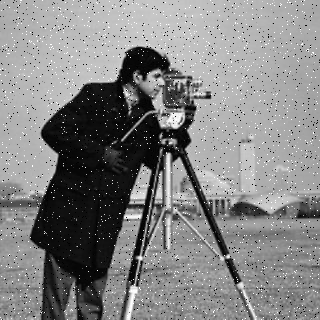
\includegraphics[width=0.5\linewidth]{Experiments/GrainRemoval/input_example.png}
	\caption{Primjerak fotografije s $5\%$ šuma soli i papra}
	\label{fig:salt_pepper_example}
\end{figure}

Postotak slike na koji sam odlučio primjeniti šum je $5\%$, slično kao i \cite{cgp_image_processing} i \cite{Sekanina2011}.
U nastavku rada također ću predstaviti rezultate na većem postotku šuma od $40\%$.

Cilj eksperimenta je evoluirati filter $f(x)$ koristeći konvolucijske metode i CGP koji će od oštećene slike $D$ reproducirati novu $Y = f(D)$ što bližu neoštećenom originalu $I$.
$$
\min_{Y, i, j} |Y_{(i, j)} - I_{(i, j)}|
$$
Iz susjedstva svake vrijednosti želimo dobiti što precizniju promatranu vrijednost. \\
Polazišna pretpostavka je ta su susjedne vrijednosti na slici u međusobnoj korelaciji do određene mjere te mogu pomoći u zaključivanju originalne vrijednosti.
Problem koji se može javiti je da u promatranom susjedstvu također imamo vrijednost koja je šum što narušava pretpostavku korelacije.
Navedeni problem je zanemaren te je CGP-u ostavljeno kao problem koji treba riješiti bez ljudskog znanja.

Jezgra $\omega$ koju sam odlučio koristiti je veličine $3 \times 3$ koja promatra $Moore$-ovo susjedstvo (\cite{jakobovic}).

\[
	\omega_{(i, j)}
	=
	\begin{bmatrix}
		x_{(i - 1, j - 1)} && x_{(i - 1, j)} && x_{(i - 1, j + 1)}\\
		x_{(i, j - 1)} && && x_{(i, j + 1)}\\
		x_{(i + 1, j - 1)} && x_{(i + 1, j)} && x_{(i + 1, j + 1)}
	\end{bmatrix}
\]
Razmišljanje iza korištenja jezgre koja ne koristi središnju, promatranu vrijednost je što tu vrijednost upravo pokušavamo predvidjeti i njena vrijednost, posebice ako je šum ne smije imati utjecaja.
Detaljniji prikaz djelovanja i rezultata mooreove jezgre vidljiv je na ilustraciji \ref{fig:moore_example}

\begin{figure}
	\centering
	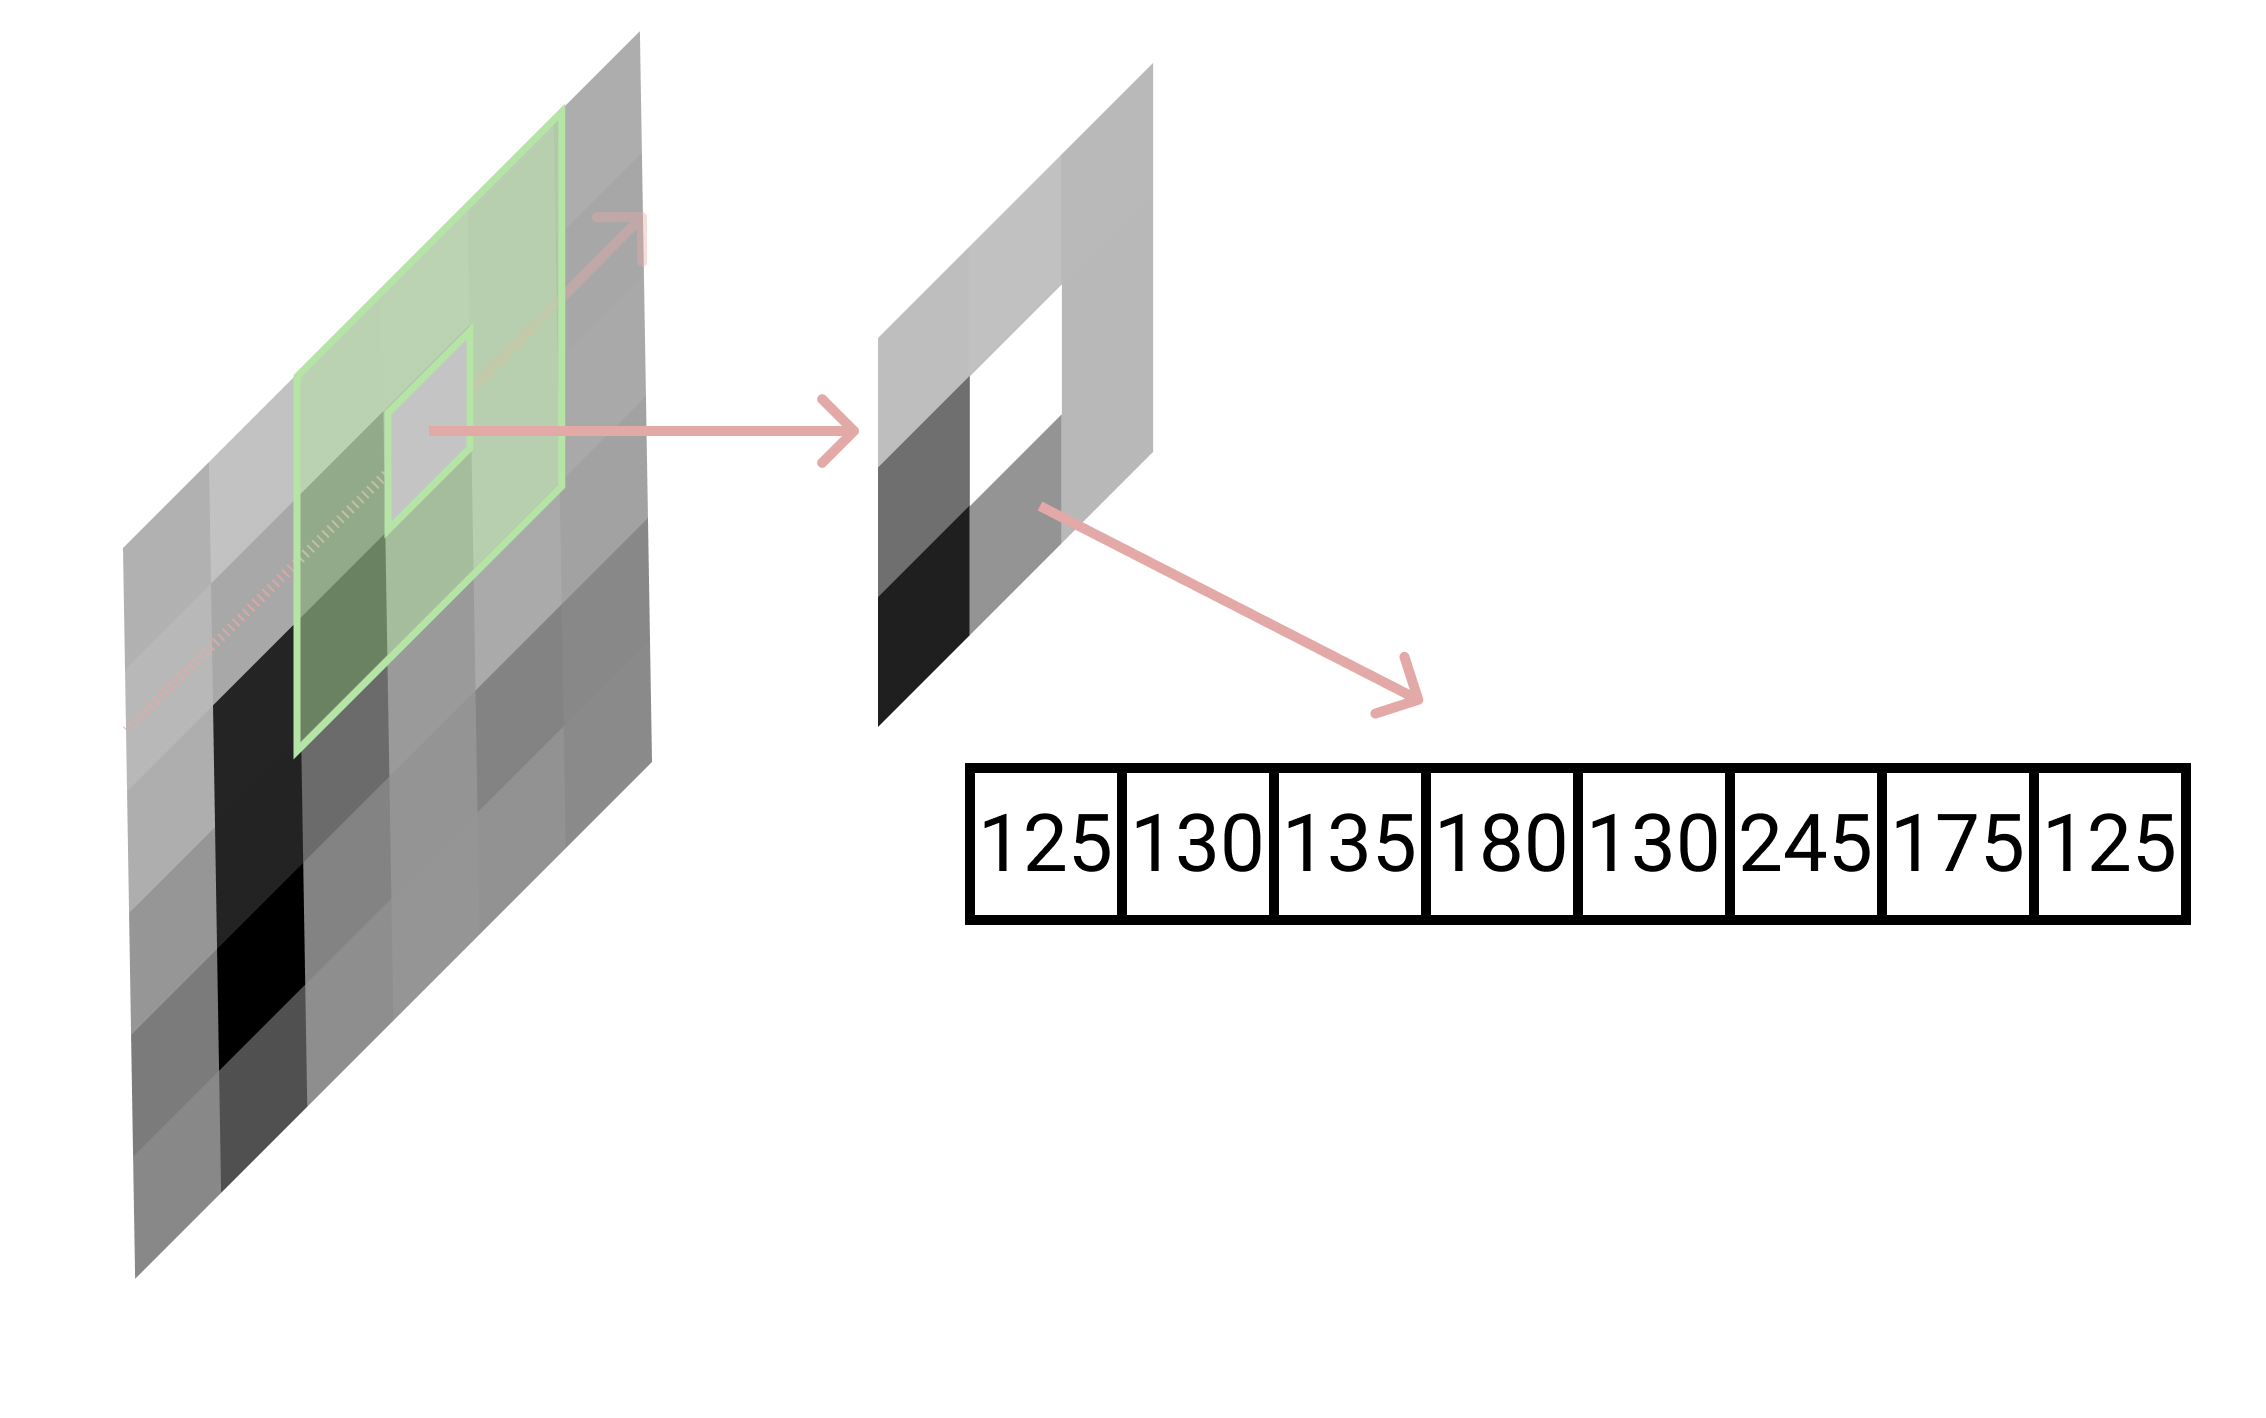
\includegraphics[width=0.8\linewidth]{Illustrations/moore.png}
	\caption{Primjer čitanja slike mooreovom jezgrom te transformacija iz preuzetog dijela slike u vektor vrijednosti koristivih CGP-u}
	\label{fig:moore_example}
\end{figure}

